\documentclass[cs6size,a4paper]{ctexart}   

%===================   导入配置信息    ===================
%==================== 数学符号公式 ============
\usepackage{amsmath}                 % AMS LaTeX宏包
\usepackage[style=1]{mdframed}
\usepackage{amsthm}
\usepackage{pdfpages}
\usepackage{amsfonts}
\usepackage{mathrsfs}                % 英文花体字 体
\usepackage{bm}                      % 数学公式中的黑斜体
\usepackage{manfnt}           % 一些图标,如 \dbend
\usepackage{lettrine}                % 首字下沉,命令\lettrine
\def\attention{\lettrine[lines=2,lraise=0,nindent=0em]{\large\textdbend\hspace{1mm}}{}}
\usepackage{longtable}
\usepackage[toc,page]{appendix}
\usepackage{geometry}                % 页边距调整
\geometry{top=3.0cm,bottom=2.7cm,left=2.5cm,right=2.5cm}
%====================公式按章编号==========================
\numberwithin{equation}{section}
\numberwithin{table}{section}
\numberwithin{figure}{section}
%================= 基本格式预置 ===========================
\usepackage{fancyhdr}
\pagestyle{fancy}
\fancyhf{}  
\fancyhead[C]{\zihao{5}  \kaishu 这是一份实验报告}
\fancyfoot[C]{~\zihao{5} \thepage~}
\renewcommand{\headrulewidth}{0.65pt} 
\CTEXsetup[format={\centering\bfseries\zihao{-2}},name={第, 章}]{section}
\CTEXsetup[nameformat={\bfseries\zihao{3}}]{subsection}
\CTEXsetup[nameformat={\bfseries\zihao{4}}]{subsubsection}

%================== 表格 =========================
\usepackage{makecell,rotating,multirow,diagbox,longtable}
%==================  图片 =========================
\newcommand{\addfig}[4][0.5]
{
  \begin{figure}[thbp!]
  \centering\includegraphics[width=#1\linewidth]{figure/#2}
  \caption{#4}
  \label{#3}
  \end{figure}
}
%================== 图形支持宏包 =========================
\usepackage{subfigure}
\usepackage{graphicx}                % 嵌入png图像
\usepackage{color,xcolor}            % 支持彩色文本、底色、文本框等
\usepackage{hyperref}                % 交叉引用
%\usepackage{caption}
\usepackage[font=small,labelfont=bf,labelsep=space]{caption}
\captionsetup{figurewithin=section}
%==================== 源码和流程图 =====================
\newcommand{\addcode}[2][None]
{
	\lstinputlisting[language=#1]{code/#2}
}

\usepackage{listings}                % 粘贴源代码
\usepackage{xcolor}
\usepackage{color}
\definecolor{dkgreen}{rgb}{0,0.6,0}
\definecolor{gray}{rgb}{0.5,0.5,0.5}
\definecolor{mauve}{rgb}{0.58,0,0.82}
\usepackage{xcolor}

\definecolor{dkgreen}{rgb}{0,0.6,0}
\definecolor{gray}{rgb}{0.5,0.5,0.5}
\definecolor{comment}{rgb}{0.56,0.64,0.68}
\lstset{
  frame=tb,
  aboveskip=3mm,
  belowskip=3mm,
  xleftmargin=2em,
  xrightmargin=2em,
  showstringspaces=false,
  keepspaces=true,
 columns=flexible,
  framerule=1pt,
  rulecolor=\color{gray!35},
  backgroundcolor=\color{gray!5},
  basicstyle={\small\ttfamily},
  numbers=none,
  numberstyle=\tiny\color{gray},
  keywordstyle=\color{blue},
  commentstyle=\color{comment},
  stringstyle=\color{dkgreen},
  breaklines=true,
  breakatwhitespace=true,
  tabsize=2,
}
% \lstset{
% breaklines=true,
%  %行号
%    numbers=left,
%     numberstyle= \tiny, 
%    basicstyle=\tiny,
%    %背景框
%    framexleftmargin=8mm,
%    frame=none,
%     %背景色
%    %backgroundcolor=\color[rgb]{1,1,0.76},
%     backgroundcolor=\color[RGB]{245,245,244},
%     %样式
%   keywordstyle=\bf\color{blue},
%   identifierstyle=\bf,
%    numberstyle=\color[RGB]{0,192,192},
%    commentstyle=\it\color[RGB]{0,96,96},
%   stringstyle=\rmfamily\slshape\color[RGB]{128,0,0},
%   %显示空格
%    showstringspaces=false
% }


%--------------------
\hypersetup{hidelinks}
\usepackage{booktabs}  
\usepackage{shorttoc}
\usepackage{tabu,tikz}
\usepackage{float}

\usepackage{multirow}



\tabcolsep=1ex
\tabulinesep=\tabcolsep
\newlength\tikzboxwidth
\newlength\tikzboxheight
\newcommand\tikzbox[1]{%
        \settowidth\tikzboxwidth{#1}%
        \settoheight\tikzboxheight{#1}%
        \begin{tikzpicture}
        \path[use as bounding box]
                (-0.5\tikzboxwidth,-0.5\tikzboxheight)rectangle
                (0.5\tikzboxwidth,0.5\tikzboxheight);
        \node[inner sep=\tabcolsep+0.5\arrayrulewidth,line width=0.5mm,draw=black]
                at(0,0){#1};
        \end{tikzpicture}%
        }

\makeatletter
\def\hlinew#1{%
  \noalign{\ifnum0=`}\fi\hrule \@height #1 \futurelet
   \reserved@a\@xhline}
   
\newcommand{\tabincell}[2]{\begin{tabular}{@{}#1@{}}#2\end{tabular}}%

\usepackage{subfigure}

\usepackage{CJK}
\usepackage{ifthen}


\usepackage{graphicx} 
\newcommand{\HRule}{\rule{\linewidth}{0.5mm}}

\newtheorem{Theorem}{定理}
\newtheorem{Lemma}{引理} 
%%使得公式随章节自动编号
\makeatletter
\@addtoreset{equation}{section}
\makeatother
\renewcommand{\theequation}{\arabic{section}.\arabic{equation}}

%-------------------------
	
\usepackage{pythonhighlight}
\usepackage{tikz}                    
\usepackage{tikz-3dplot}
\usetikzlibrary{shapes,arrows,positioning}

%===================   正文开始    ===================
\begin{document}
\bibliographystyle{gbt7714-2005}     %论文引用格式
%===================  定理类环境定义 ===================
\newtheorem{example}{例}              % 整体编号
\newtheorem{algorithm}{算法}
\newtheorem{theorem}{定理}            % 按 section 编号
\newtheorem{definition}{定义}
\newtheorem{axiom}{公理}
\newtheorem{property}{性质}
\newtheorem{proposition}{命题}
\newtheorem{lemma}{引理}
\newtheorem{corollary}{推论}
\newtheorem{remark}{注解}
\newtheorem{condition}{条件}
\newtheorem{conclusion}{结论}
\newtheorem{assumption}{假设}
%==================重定义 ===================
\renewcommand{\contentsname}{目录}     
\renewcommand{\abstractname}{摘要} 
\renewcommand{\refname}{参考文献}     
\renewcommand{\indexname}{索引}
\renewcommand{\figurename}{图}
\renewcommand{\tablename}{表}
\renewcommand{\appendixname}{附录}
\renewcommand{\proofname}{证明}
\renewcommand{\algorithm}{算法} 
%============== 封皮和前言 =================
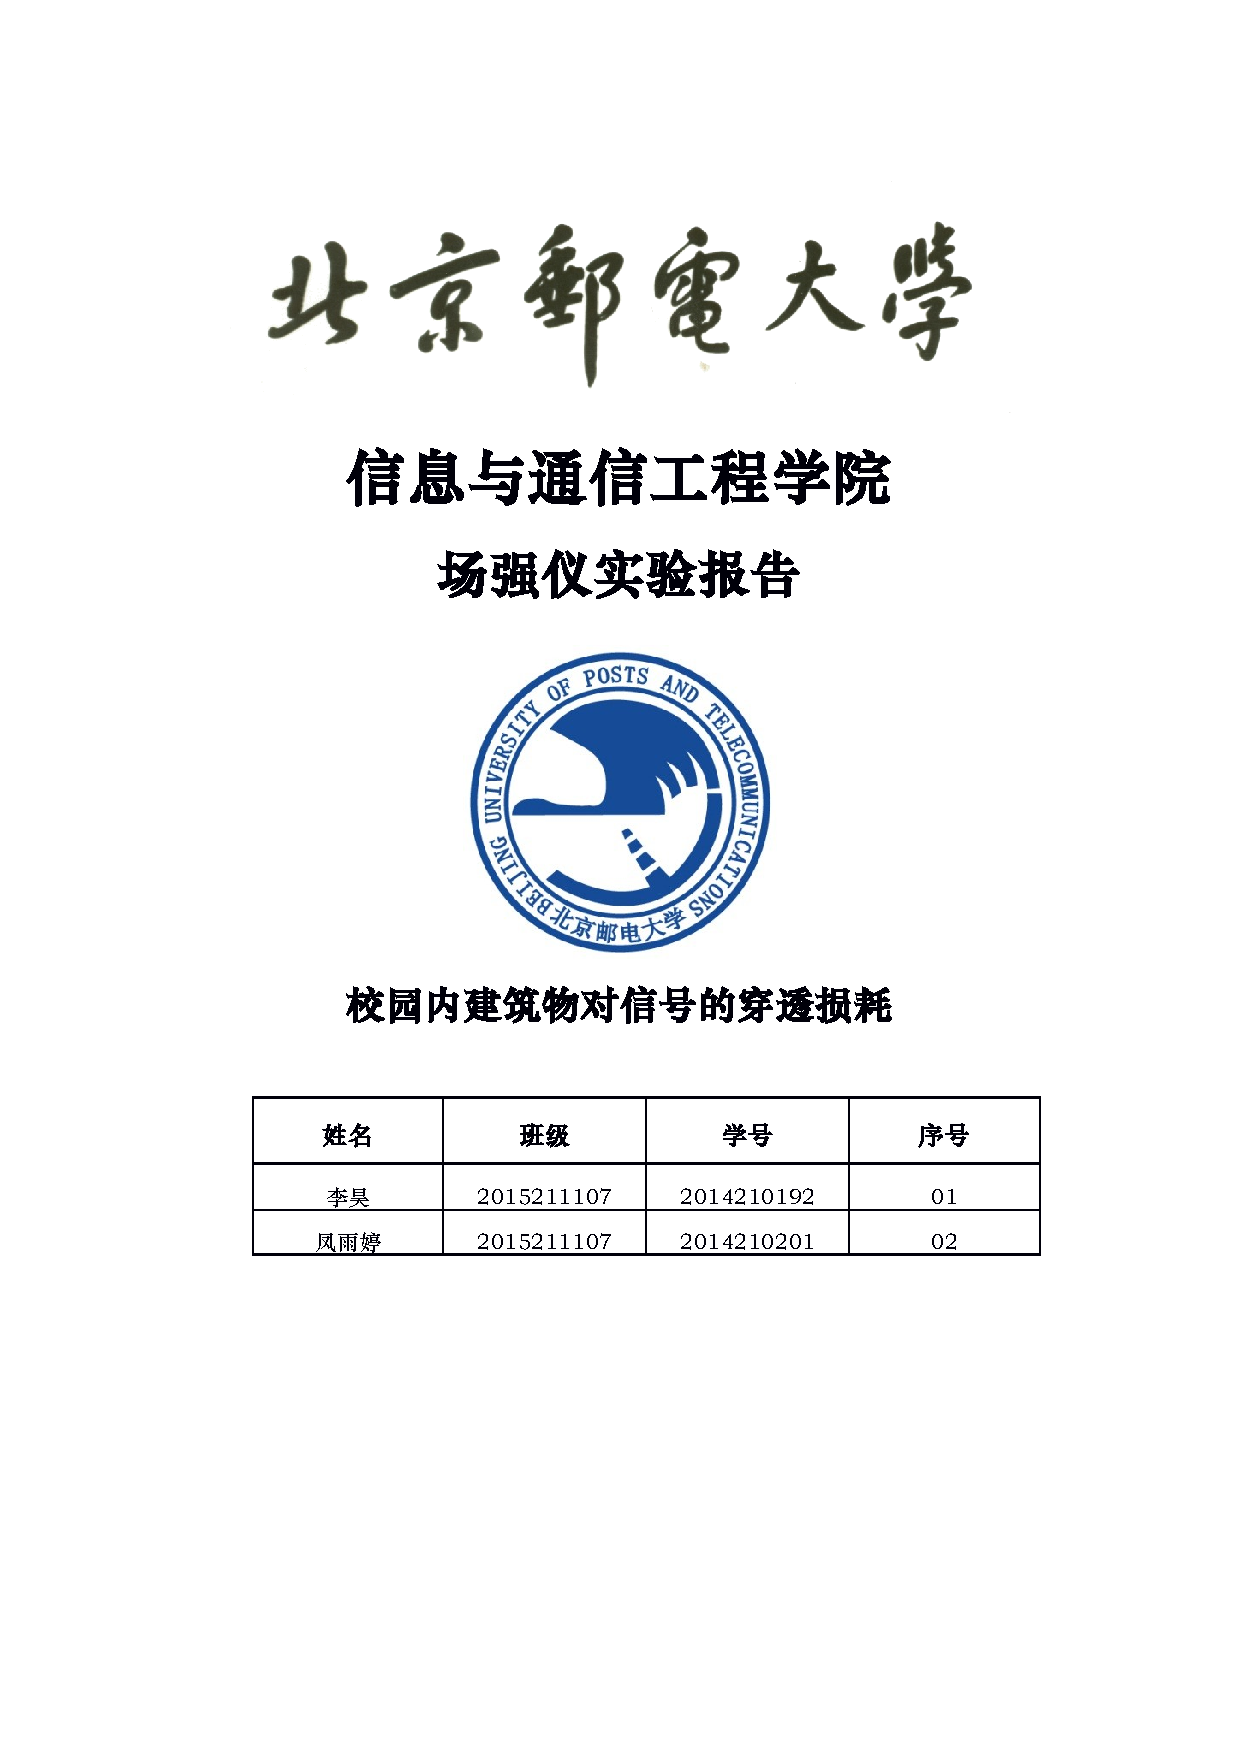
\includepdf[page=1]{cover/cover}
\pagestyle{plain}
\pagenumbering{roman}
%\section*{\zihao{3} \centering 摘要}

\vskip0.5cm
本文旨在通过用场强仪测量校园内信号的真实数据来总结衰落的规律

\textbf{关键词:} 场强仪, 穿透衰落
\addcontentsline{toc}{section}{摘要}

\clearpage
%\section*{\zihao{2} \centering \textbf{Abstract} }
%   %用了Times New Roman字体来美化观感
%Our design aimed at simulating the network environment of a campus network with a minimum number of equipments.
%On the point of connection function,all of our inside hosts can visit the Internet.What'more,the server is open to
%both the intranet and the outer network.In terms of security ,what we have already relized is the isolation between
%different departments but interoperability,isolation of teaching and non teaching areas.AS  for IP allocation,
%the server is allocated in a static IP, and the other terminals are allocated with dynamic IP.Also,there are three services:campus web site,file sharing and internal network DNS.  
%
%\textbf{Key Words:}Campus network ,ACL ,VLAN ,DHCP ,NAT ,DNS 
%\addcontentsline{toc}{section}{Abstract}
%
%
%
%

%\pagestyle{empty}
\tableofcontents 
%\thispagestyle{empty}
%============== 论文正文   =================
\pagestyle{fancy}
\pagenumbering{arabic}

\section{实验背景}
	\subsection{实验目的}
		通过测量实际数据研究校园内建筑物的穿透损耗
	\subsection{数据的选择与说明}
		\begin{description}
		  \item{\textbf{测量地点}} 教二,教一的南北两侧,各自西向东100个点, 主楼前广场南北两侧各自西向东50个点, 一共500个点
		  \item{\textbf{测量频率}} 我们选择中国之声FM, 频率为106.1MHz
		  \item{\textbf{测量方式}} 场强仪电线指向西边, 水平向上45度
		  \item{\textbf{测量步长}} 约为1米
		  \item{\textbf{测量状态}} 2018年4月24日, 15:30-14:30, 大风, 晴
		  \item{\textbf{绘图工具}} python+jupyter+matplotlib+pandas
		  \item{\textbf{源代码}} 托管在我的github\cite{mygithub}
		\end{description}
	

      %
\pagenumbering{arabic}

\section{数据分析}

 	\subsection{全局分析}
	图\ref{fig:all}展示的是信号强度在二位地理位置上的分布.
	图中的四个红色的框分别代表教一, 主楼, 广场, 教二.
	通过右边的colormap可以直观的感受到信号在地理分布上的规律.
	\addfig[0.8]{all.png}{fig:all}{全局分析}  

 \indent	从中可以看到如下事实
	  \begin{enumerate}
		\item 对于教二和教一来说, 南边的信号要比北边要强, 猜测信号源在学校的北边
		\item 广场的信号分布相对均匀一些, 猜测是因为广场空间宽阔
		\item 教一南到广场北和广场南到教二北有明显衰减, 猜测是因为广场周边的树造成的
	  \end{enumerate}
	
 	\subsection{南北分析}
	为了分析信号在南北方向的分布规律, 我们把所有点在东西方向去平均, 得到图\ref{fig:sourth-north}
	图中"oneS"代表教一南, "squareN"代表广场北
	\addfig[0.8]{sorth-north.png}{fig:sourth-north}{南北分析}

 \indent	从中可以看到如下事实
		\begin{enumerate}
		  \item 对于一个实体(广场, 教一, 教二), 南面信号比北面强, 猜测是因为信号源在学校南方
		  \item	教二北比广场南的信号要弱, 这是唯一一个违背南强北弱规律的, 暂时无法解释
		\end{enumerate}

 \indent	求平均后的数据如表\ref{table:sourth-north-mean}
	\begin{table}[htbp]
\centering
\begin{tabular}{lllllll}
 \toprule
   & twoS    & twoN    & squareS & squareN & oneS    & oneN   \\ 
 \midrule
数据 & -58.732 & -59.688 & -57.94  & -58.968 & -59.746 & -61.19 \\ 
\bottomrule
\end{tabular}
\caption{南北方向平均值}
\label{table:sourth-north-mean}
\end{table}


 \indent	根据衰落计算公式$$\Delta P = \frac{1}{N} \sum _{i=1} ^{N} P_i^{outside} -\frac{1}{M} \sum _{j=1} ^{M} P_j^{inside}$$可以得到表\ref{table:sorth-north-delta}
	\begin{table}[htbp]
\centering
\begin{tabular}{ll}
\toprule 
                & 衰落损耗   \\ 
\midrule
twoS-twoN       & 0.965  \\     
towN-squareS    & -1.748 \\     
squareS-squareN & 1.028  \\     
squareN-oneS    & 0.778  \\     
oneS-oneN       & 1.444 \\
\bottomrule
\end{tabular}
\caption{南北方向衰落损耗}
  \label{table:sorth-north-delta}
\end{table}


 	\subsection{东西分析}
	为了分析信号在东西方向的分布规律, 我们把所有的点在南北方向上取平均, 得到图\ref{fig:west-east}
	图中x轴代表自西像东的第x个点
	\addfig[0.8]{west-east.png}{fig:west-east}{东西分析}
\\\indent	计算其统计特性可以得到表\ref{table:west-east-statistic}
	\begin{table}[htbp]
\centering
\begin{tabular}{lll}
  \toprule
       & mean       & std      \\
	 \midrule
result & -59.601250 & 2.126018\\
\bottomrule
\end{tabular}
\caption{东西方向的统计特性}
  \label{table:west-east-statistic}
\end{table}

	

      %
%\include{body/table}
%\pagenumbering{arabic}

\section{实验背景}
	\subsection{实验目的}
		通过测量实际数据研究校园内建筑物的穿透损耗
	\subsection{数据的选择与说明}
		\begin{description}
		  \item{\textbf{测量地点}} 教二,教一的南北两侧,各自西向东100个点, 主楼前广场南北两侧各自西向东50个点, 一共500个点
		  \item{\textbf{测量频率}} 我们选择中国之声FM, 频率为106.1MHz
		  \item{\textbf{测量方式}} 场强仪电线指向西边, 水平向上45度
		  \item{\textbf{测量步长}} 约为1米
		  \item{\textbf{测量状态}} 2018年4月24日, 15:30-14:30, 大风, 晴
		  \item{\textbf{绘图工具}} python+jupyter+matplotlib+pandas
		  \item{\textbf{源代码}} 托管在我的github\cite{mygithub}
		\end{description}
	

      %
%============= 参考文献 =====================
%\addcontentsline{toc}{section}{参考文献}
\begin{thebibliography}{9}
\bibitem{mygithub} 
  github of lihao2333, 李昊, \url{git@github.com:lihao2333/HW_RADIO.git}
\end{thebibliography}
\clearpage


%=============  致谢  ======================
%\section*{致谢}
\addcontentsline{toc}{section}{致谢}
感谢父母为我提供的良好的衣食条件,让我有精力投入到这项没有经济回报的项目中去。
感谢徐海祥老师为我定制的论文题目,这个题目让我有兴趣制作这个模板。感谢武汉理工大学博士与硕士论文作者Hu,Weiyi,我在本模板制作的过程中参考了前辈的思路的方法。我研究过的模板还包括:上海交通大学,清华大学,哈尔滨工业大学,以及中国科技大学。其中论文引用格式GBT7714-2005-BibTeX-Style是上海财经大学的Haixing Hu作品,本模板离不开这些有益的资源的支持。同样感谢正在使用这个模板的你,相信通过你们的使用和传播,这个模板会变得越来越完善。
\newpage
\appendix
%%附录第一个章节
\section{原始数据}
下表为原始数据, 注意没有负号

\begin{longtable}{lllllll}
  \toprule
    & twoS & twoN & squareS & squareN & oneS & oneN \\
	\midrule
1   & 61.8 & 62.6 & 60.9    & 56.8    & 65.5 & 58   \\
2   & 55.1 & 57.6 & 62.5    & 64.8    & 60.2 & 57.5 \\
3   & 54.9 & 58.8 & 71.6    & 62.7    & 60.3 & 58.8 \\
4   & 60.1 & 59.1 & 58.4    & 66.7    & 59.4 & 57.3 \\
5   & 53.7 & 65.5 & 55.4    & 61.7    & 55.3 & 58.4 \\
6   & 53.1 & 68.4 & 56.6    & 62.8    & 56.8 & 58.7 \\
7   & 60.9 & 69.3 & 63.1    & 65.3    & 64.2 & 61   \\
8   & 62.7 & 63.4 & 57.2    & 60.2    & 57.2 & 59.7 \\
9   & 61.2 & 59.9 & 58.5    & 60.3    & 65.8 & 63.4 \\
10  & 54.6 & 67.2 & 58.6    & 56.1    & 61.6 & 58.2 \\
11  & 59.5 & 62.8 & 54.8    & 65.1    & 55.9 & 57.1 \\
12  & 60.5 & 64.5 & 61.5    & 54.9    & 59.8 & 58.3 \\
13  & 54.4 & 66.3 & 63      & 62.8    & 61.1 & 59.3 \\
14  & 51.8 & 61.3 & 57      & 56.8    & 58.2 & 59.6 \\
15  & 56.3 & 69.9 & 58.3    & 58.4    & 61.7 & 59.9 \\
16  & 54.6 & 58.3 & 59.2    & 56.6    & 64.7 & 57.5 \\
17  & 59   & 62.5 & 60.5    & 53.8    & 63.7 & 61   \\
18  & 57.3 & 63.6 & 60.2    & 62.3    & 64.5 & 55.4 \\
19  & 55.4 & 57   & 57.3    & 56      & 58.9 & 56.8 \\
20  & 53.5 & 70.2 & 64.8    & 56.8    & 70.4 & 68.9 \\
21  & 50.6 & 58.7 & 60.4    & 62.8    & 60.5 & 57.8 \\
22  & 57.9 & 62.6 & 57.7    & 59.3    & 58.8 & 52   \\
23  & 53.5 & 60.2 & 64.8    & 56.8    & 62.5 & 58.3 \\
24  & 54.6 & 61.3 & 62.9    & 57.6    & 58.1 & 59.9 \\
25  & 57   & 58.7 & 56.4    & 61.5    & 61.6 & 61.5 \\
26  & 56.8 & 59.3 & 59.4    & 58.2    & 60.9 & 62.6 \\
27  & 65.1 & 56   & 55.3    & 53.7    & 56.6 & 64.9 \\
28  & 60.4 & 55.8 & 50.7    & 57      & 54.4 & 61.6 \\
29  & 60.9 & 60.5 & 60.5    & 61.2    & 53.5 & 60.3 \\
30  & 62.1 & 62.7 & 49.4    & 58.7    & 57.9 & 59.8 \\
31  & 63.8 & 63.8 & 49.3    & 62.5    & 60.6 & 60.5 \\
32  & 55.6 & 60.8 & 55.4    & 57.9    & 60.8 & 61.3 \\
33  & 57.8 & 65.7 & 48.1    & 52.7    & 54.8 & 60.9 \\
34  & 60.6 & 56.6 & 52.4    & 64.4    & 52.9 & 64.8 \\
35  & 55.1 & 54.1 & 49      & 54.8    & 58.9 & 64.3 \\
36  & 57.6 & 61.5 & 51      & 55.7    & 61.1 & 62.9 \\
37  & 58.8 & 56.6 & 53.5    & 58.6    & 56.6 & 60.7 \\
38  & 55.4 & 54.8 & 51.2    & 55.2    & 62.3 & 60.2 \\
39  & 59.9 & 59.9 & 60.5    & 57.6    & 60.6 & 67.8 \\
40  & 72.4 & 59.2 & 52.8    & 64.5    & 55.9 & 65.8 \\
41  & 53.7 & 63.4 & 54.4    & 63.6    & 60.9 & 60.7 \\
42  & 52.7 & 70.3 & 64.2    & 56.8    & 62.7 & 60.2 \\
43  & 56.3 & 66.6 & 55.5    & 56.8    & 56.8 & 60.5 \\
44  & 59.5 & 67.1 & 57.2    & 62.5    & 55.8 & 62.2 \\
45  & 50.2 & 65.1 & 67.1    & 56.9    & 68.8 & 56.1 \\
46  & 48.7 & 65.8 & 55.7    & 51.5    & 64.4 & 59.7 \\
47  & 61.5 & 65.1 & 57.3    & 52.8    & 60.6 & 45.2 \\
48  & 55.5 & 60.8 & 62.1    & 60.1    & 60.9 & 60.4 \\
49  & 51.1 & 57.5 & 69.2    & 60.4    & 56.5 & 58.5 \\
50  & 59.7 & 69.3 & 54.2    & 55.4    & 59.4 & 65.4 \\
51  & 56.1 & 63.4 & 0       & 0       & 65.1 & 60.6 \\
52  & 57.1 & 65.2 & 0       & 0       & 60.2 & 59.3 \\
53  & 64.3 & 60.8 & 0       & 0       & 55.4 & 62.8 \\
54  & 59.5 & 61.3 & 0       & 0       & 57.7 & 62.5 \\
55  & 56.7 & 60.8 & 0       & 0       & 60.7 & 60   \\
56  & 60.5 & 60.1 & 0       & 0       & 68.5 & 58.8 \\
57  & 52.7 & 57.8 & 0       & 0       & 58.8 & 60.4 \\
58  & 53.7 & 50.7 & 0       & 0       & 53.5 & 59.1 \\
59  & 56.4 & 55.1 & 0       & 0       & 55.9 & 65.5 \\
60  & 52.9 & 57.7 & 0       & 0       & 64.1 & 66.4 \\
61  & 60.3 & 58.9 & 0       & 0       & 60.5 & 60.4 \\
62  & 59.3 & 51.9 & 0       & 0       & 59.9 & 58.6 \\
63  & 55.5 & 52.4 & 0       & 0       & 62.2 & 65.9 \\
64  & 50.2 & 52.8 & 0       & 0       & 62.7 & 66.1 \\
65  & 47.4 & 52.9 & 0       & 0       & 62.5 & 64.5 \\
66  & 49.3 & 58.7 & 0       & 0       & 66.4 & 69.6 \\
67  & 54.1 & 64.5 & 0       & 0       & 61.9 & 69.5 \\
68  & 71.1 & 57.9 & 0       & 0       & 62.7 & 61.7 \\
69  & 64.1 & 50.4 & 0       & 0       & 61.1 & 60.8 \\
70  & 67.1 & 54.6 & 0       & 0       & 61   & 62.1 \\
71  & 60.3 & 51   & 0       & 0       & 60.5 & 60.4 \\
72  & 58   & 52   & 0       & 0       & 60.4 & 68.6 \\
73  & 59.7 & 55.5 & 0       & 0       & 61.2 & 57.4 \\
74  & 53.1 & 51.3 & 0       & 0       & 55.1 & 59.8 \\
75  & 51.4 & 52.1 & 0       & 0       & 54.9 & 67.8 \\
76  & 62.2 & 54.3 & 0       & 0       & 55.6 & 64.7 \\
77  & 59.6 & 52.6 & 0       & 0       & 53.3 & 66   \\
78  & 71.3 & 63.1 & 0       & 0       & 52.7 & 56.8 \\
79  & 65   & 56.4 & 0       & 0       & 54.2 & 61.9 \\
80  & 61.8 & 56.8 & 0       & 0       & 57.5 & 56.8 \\
81  & 58.8 & 55   & 0       & 0       & 62.9 & 58   \\
82  & 71.9 & 53.6 & 0       & 0       & 61.7 & 63.6 \\
83  & 65.3 & 59.7 & 0       & 0       & 59.8 & 60.5 \\
84  & 61.2 & 50.8 & 0       & 0       & 56.6 & 56.2 \\
85  & 58.9 & 51.5 & 0       & 0       & 54.7 & 64   \\
86  & 71.3 & 55.5 & 0       & 0       & 54.6 & 58.7 \\
87  & 62.4 & 55.9 & 0       & 0       & 55.7 & 58   \\
88  & 57.1 & 55.6 & 0       & 0       & 56.7 & 62.5 \\
89  & 58.5 & 58.8 & 0       & 0       & 57.5 & 61.8 \\
90  & 59.9 & 65.7 & 0       & 0       & 53.9 & 58.7 \\
91  & 61.5 & 67.1 & 0       & 0       & 57.9 & 61.5 \\
92  & 65   & 62.7 & 0       & 0       & 58.2 & 61.9 \\
93  & 62.4 & 63.2 & 0       & 0       & 75.6 & 71.9 \\
94  & 70.4 & 55.6 & 0       & 0       & 58.9 & 65.5 \\
95  & 60.6 & 53.7 & 0       & 0       & 57.9 & 61.5 \\
96  & 60.1 & 56.8 & 0       & 0       & 60.2 & 60.4 \\
97  & 67.6 & 62.7 & 0       & 0       & 57.6 & 62.2 \\
98  & 63.8 & 63.1 & 0       & 0       & 57.4 & 64.8 \\
99  & 63   & 59.3 & 0       & 0       & 67.2 & 63.5 \\
100 & 57.6 & 61.5 & 0       & 0       & 62.1 & 67.4 \\
\bottomrule

\end{longtable}

%============= 工作日志  ===================
%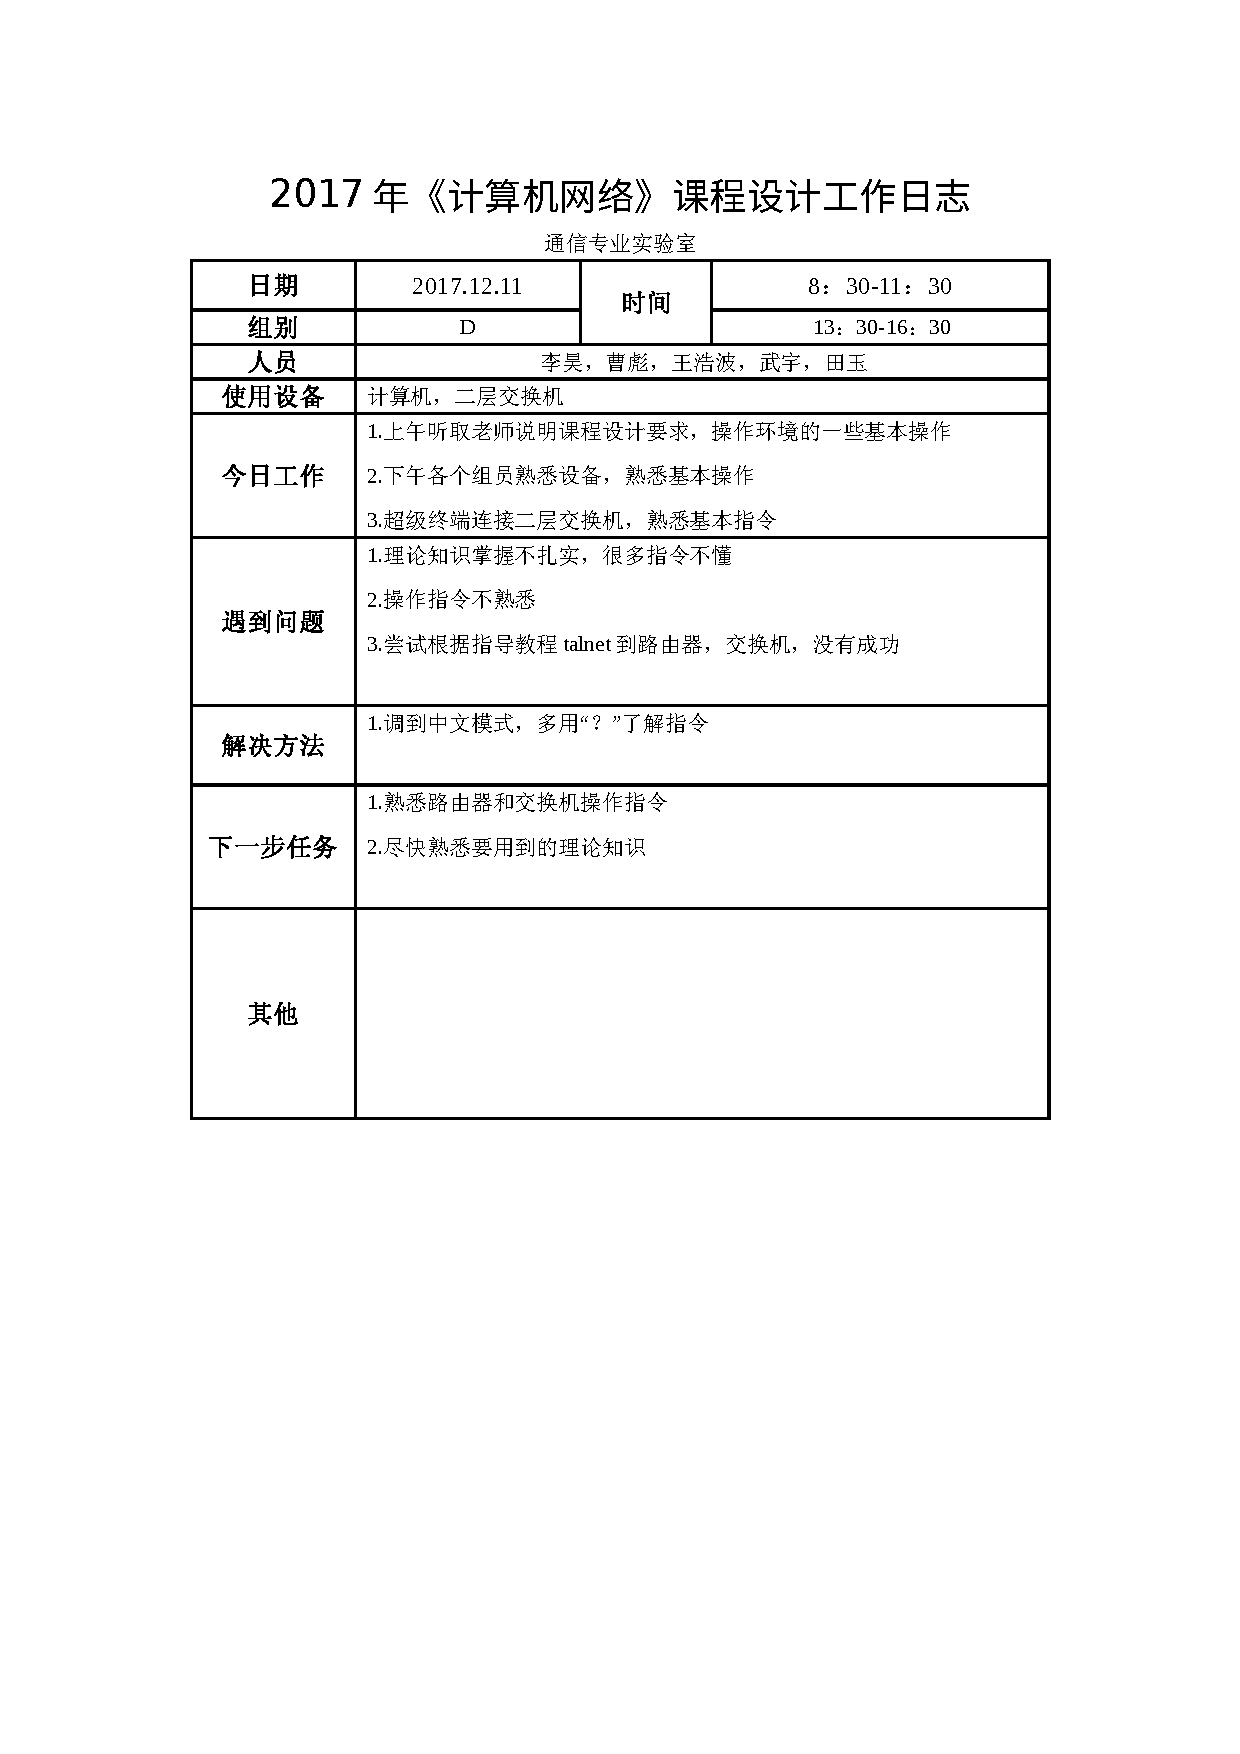
\includepdf[pages=1-10]{body/log}

\end{document}
%%%%%%%%%% 结束 %%%%%%%%%%
